\documentclass[10pt,a4paper,twocolumn]{article}

% ── Encoding & Language ──────────────────────────────────────────────────────
\usepackage[utf8]{inputenc}
\usepackage[T1]{fontenc}

% ── Layout ───────────────────────────────────────────────────────────────────
\usepackage[top=2.3cm, bottom=2.3cm, left=2.0cm, right=2.0cm]{geometry}
\usepackage{setspace}
\setstretch{1.08}
\usepackage{indentfirst}
\setlength{\parindent}{1.25cm}
\setlength{\parskip}{0pt}
\setlength{\columnsep}{0.7cm}
\setlength{\emergencystretch}{3em}

% ── Fonts & Typography ───────────────────────────────────────────────────────
\usepackage{lmodern}
\usepackage{microtype}

% ── Graphics & Tables ────────────────────────────────────────────────────────
\usepackage{graphicx}
\usepackage{booktabs}
\usepackage{caption}
\usepackage{subcaption}
\usepackage{float}
\usepackage{array}
\usepackage{xcolor}
\usepackage{tabularx}
\usepackage{dblfloatfix}

% ── Math ─────────────────────────────────────────────────────────────────────
\usepackage{amsmath}

% ── Hyperlinks ───────────────────────────────────────────────────────────────
\usepackage[hidelinks,hypertexnames=false]{hyperref}
\renewcommand{\contentsname}{Sumário}

% ── Headers & Footers ────────────────────────────────────────────────────────
\usepackage{fancyhdr}
\pagestyle{fancy}
\fancyhf{}
\fancyhead[L]{\small Laboratório de Experimentação de Software}
\fancyhead[R]{\small PUC Minas -- 2026/1}
\fancyfoot[C]{\thepage}
\setlength{\headheight}{14pt}
\renewcommand{\headrulewidth}{0.4pt}

% ─────────────────────────────────────────────────────────────────────────────
\begin{document}

\onecolumn

% ── Capa ─────────────────────────────────────────────────────────────────────
\begin{titlepage}
  \centering
  \vspace*{2.0cm}

  {\normalsize
    Pontifícia Universidade Católica de Minas Gerais (PUC~Minas)\\
    Laboratório de Experimentação de Software -- 2026/1
  }

  \vspace*{2.8cm}

  {\large
    Raphael Brito\\[0.3em]
    Yan Cota
  }

  \vspace*{4.2cm}

  {\LARGE \textbf{Laboratório 03}\\[0.5em]
  \Large Caracterizando a Atividade de Code Review no GitHub}

  \vfill

  {\normalsize Belo Horizonte\\ 2026}
\end{titlepage}

% ── Sumário ──────────────────────────────────────────────────────────────────
\pagenumbering{roman}
\tableofcontents
\newpage
\pagenumbering{arabic}
\setcounter{page}{1}
\twocolumn

% ─────────────────────────────────────────────────────────────────────────────
\section{Introdução}
% ─────────────────────────────────────────────────────────────────────────────

O processo de \textit{code review} -- revisão formal de código por pares -- é
amplamente reconhecido como uma das práticas mais efetivas para garantir
qualidade e disseminar conhecimento em projetos de software.
Plataformas como o GitHub popularizaram o modelo de \textit{pull requests}
(PRs), em que uma contribuição passa por discussão e aprovação antes de ser
integrada ao código principal.

Neste laboratório analisamos \textbf{17.543\,\textit{pull requests}}
coletados dos \textbf{200 repositórios mais populares} do GitHub (medidos
por número de estrelas), investigando como características dos PRs se
relacionam com seu desfecho final (\textit{merged} ou \textit{closed}) e com
o volume de revisões recebidas.

\section{Questões de Pesquisa e Hipóteses}

Antes de analisar os dados, levantamos as seguintes hipóteses:

\begin{description}
  \item[\textbf{H$_{\text{A}}$ -- Características e status final}]
    Esperamos que PRs \textit{merged} apresentem menor número de arquivos
    alterados, menor tamanho de diff e descrições mais completas, pois
    mudanças bem documentadas e de escopo reduzido tendem a ser aceitas com
    mais facilidade pelos revisores.

  \item[\textbf{H$_{\text{B}}$ -- Características e número de revisões}]
    Esperamos que PRs com mais participantes e comentários também recebam
    mais revisões formais, pois discussões ativas costumam envolver ciclos
    iterativos de revisão.
\end{description}

% ─────────────────────────────────────────────────────────────────────────────
\section{Objetivos}
% ─────────────────────────────────────────────────────────────────────────────

\subsection{Objetivo Geral}

Caracterizar a atividade de \textit{code review} nos repositórios mais
populares do GitHub, identificando fatores associados à aprovação de PRs e
ao volume de revisões recebidas.

\subsection{Objetivos Específicos}

\begin{itemize}
  \item Comparar distribuições de métricas de PRs entre os grupos MERGED e
    CLOSED usando o teste de Mann-Whitney~U.
  \item Correlacionar características dos PRs com o número de revisões
    recebidas via coeficiente de Spearman.
  \item Identificar quais fatores estão mais fortemente associados ao
    desfecho e ao engajamento no processo de revisão.
\end{itemize}

% ─────────────────────────────────────────────────────────────────────────────
\section{Metodologia}
% ─────────────────────────────────────────────────────────────────────────────

\subsection{Coleta de Dados}

A coleta foi realizada em duas etapas:

\begin{enumerate}
  \item \textbf{Seleção de repositórios:} via \textbf{API GraphQL do GitHub},
    coletamos os 200 repositórios mais populares (por estrelas),
    filtrando aqueles com no mínimo 100 PRs mergeados ou fechados.

  \item \textbf{Coleta de PRs:} para cada repositório foram coletados os
    últimos PRs com status \textit{MERGED} ou \textit{CLOSED}, registrando:
    número de arquivos alterados, linhas adicionadas e removidas, tempo de
    revisão (horas entre abertura e encerramento), tamanho da descrição
    (em caracteres), número de participantes, de comentários e de revisões
    formais.
\end{enumerate}

O dataset final contém 17.543 PRs: 12.287 MERGED e
5.256 CLOSED.

\subsection{Análise}

\paragraph{RQ$_A$ -- Status do PR.}
Distribuições de cada métrica nos grupos MERGED e CLOSED foram comparadas
com o \textbf{teste de Mann-Whitney~U} (bicaudal), não-paramétrico e robusto
a outliers. Significância: $p < 0{,}001$ (***), $p < 0{,}01$ (**),
$p < 0{,}05$ (*) e $p \geq 0{,}05$ (ns).

\paragraph{RQ$_B$ -- Número de revisões.}
Para cada métrica calculamos o \textbf{coeficiente de correlação de
Spearman} ($\rho$) em relação ao número de revisões formais do PR.

% ─────────────────────────────────────────────────────────────────────────────
\section{Resultados}
% ─────────────────────────────────────────────────────────────────────────────

A Tabela~\ref{tab:medians} apresenta as medianas globais de cada métrica.

\begin{table}[H]
  \centering
  \caption{Medianas globais das métricas de PRs.}
  \label{tab:medians}
  \begin{tabular}{lr}
    \toprule
    \textbf{Métrica} & \textbf{Mediana} \\
    \midrule
    Arquivos alterados & 1,00 \\
    Adições (linhas) & 11,00 \\
    Deleções (linhas) & 2,00 \\
    Tempo de revisão (h) & 49,76 \\
    Tamanho da descrição & 826,00 \\
    Participantes & 3,00 \\
    Comentários & 2,00 \\
    \bottomrule
  \end{tabular}
\end{table}

% ─────────────────────────────────────────────────────────────────────────────
\subsection{RQ$_A$ -- Relação entre características e status final}
% ─────────────────────────────────────────────────────────────────────────────

A Tabela~\ref{tab:rqa} resume os resultados do teste de Mann-Whitney~U.
Todas as métricas apresentaram diferença significativa ($p < 0{,}001$).
A coluna \textbf{Tend.} indica se PRs MERGED (M) têm valores maiores ou
menores que CLOSED (C).

\begin{table}[H]
  \centering
  \caption{Mann-Whitney U: MERGED vs.\ CLOSED. Todas as diferenças com $p<0{,}001$ (***).}
  \label{tab:rqa}
  \small
  \begin{tabular}{lll}
    \toprule
    \textbf{Métrica} & \textbf{Sig.} & \textbf{Tend.} \\
    \midrule
    Arquivos alterados & *** & M $>$ C \\
    Adições (linhas) & *** & M $>$ C \\
    Deleções (linhas) & *** & M $>$ C \\
    Tempo de revisão (h) & *** & M $<$ C \\
    Tamanho da descrição & *** & M $<$ C \\
    Participantes & *** & M $<$ C \\
    Comentários & *** & M $<$ C \\
    \bottomrule
  \end{tabular}
\end{table}

Os boxplots a seguir comparam as distribuições de cada métrica entre os
dois grupos. Cada par de figuras é identificado com a significância e a
direção da diferença:

\begin{figure}[H]
  \centering
  \begin{subfigure}[b]{0.48\columnwidth}
    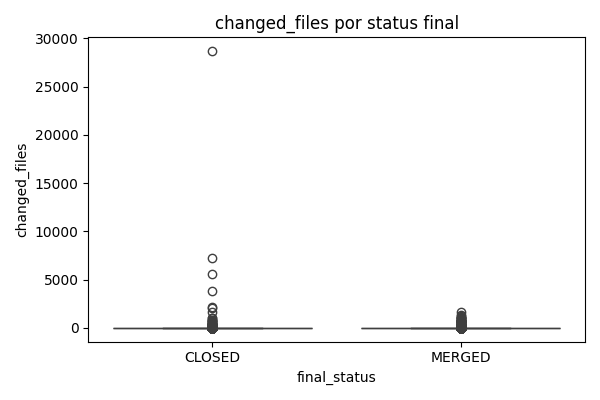
\includegraphics[width=\textwidth]{figs/box_changed_files.png}
    \caption{Arquivos alterados (***; MERGED $>$ CLOSED)}
  \end{subfigure}
  \hfill
  \begin{subfigure}[b]{0.48\columnwidth}
    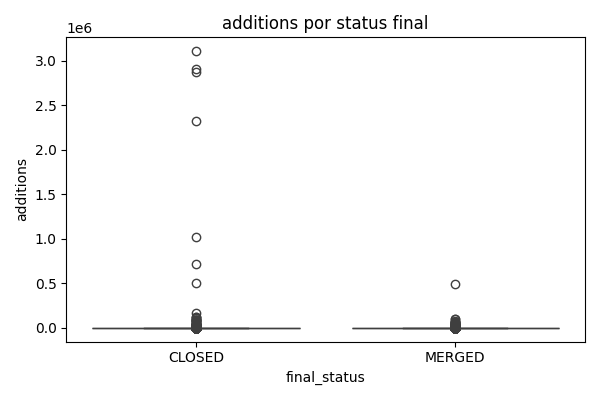
\includegraphics[width=\textwidth]{figs/box_additions.png}
    \caption{Adições (linhas) (***; MERGED $>$ CLOSED)}
  \end{subfigure}
  \caption{Distribuição por status (MERGED vs.\ CLOSED). Sig.: *** $p<0{,}001$. M\,=\,MERGED, C\,=\,CLOSED}
  \label{fig:box1}
\end{figure}

\begin{figure}[H]
  \centering
  \begin{subfigure}[b]{0.48\columnwidth}
    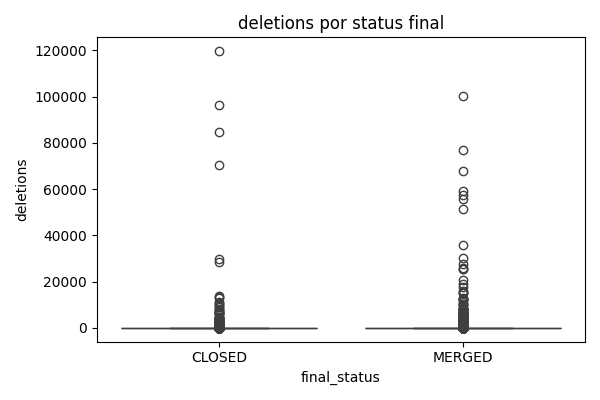
\includegraphics[width=\textwidth]{figs/box_deletions.png}
    \caption{Deleções (linhas) (***; MERGED $>$ CLOSED)}
  \end{subfigure}
  \hfill
  \begin{subfigure}[b]{0.48\columnwidth}
    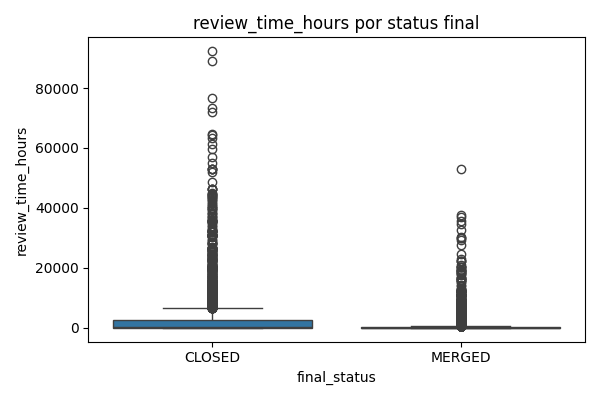
\includegraphics[width=\textwidth]{figs/box_review_time_hours.png}
    \caption{Tempo de revisão (h) (***; MERGED $<$ CLOSED)}
  \end{subfigure}
  \caption{Distribuição por status (MERGED vs.\ CLOSED). Sig.: *** $p<0{,}001$. M\,=\,MERGED, C\,=\,CLOSED (cont.)}
  \label{fig:box2}
\end{figure}

\begin{figure}[H]
  \centering
  \begin{subfigure}[b]{0.48\columnwidth}
    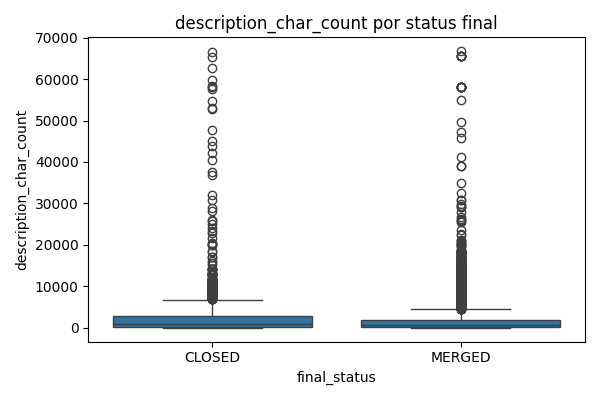
\includegraphics[width=\textwidth]{figs/box_description_char_count.png}
    \caption{Tamanho da descrição (***; MERGED $<$ CLOSED)}
  \end{subfigure}
  \hfill
  \begin{subfigure}[b]{0.48\columnwidth}
    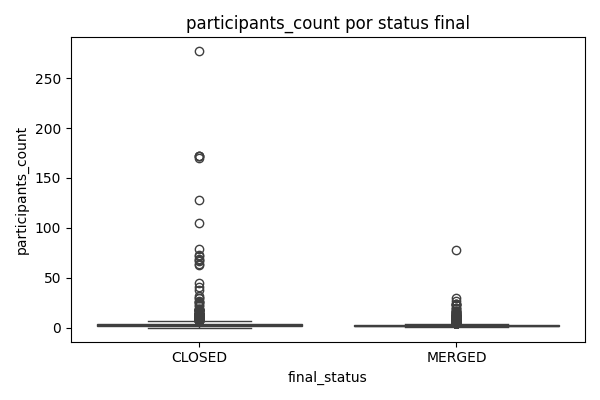
\includegraphics[width=\textwidth]{figs/box_participants_count.png}
    \caption{Participantes (***; MERGED $<$ CLOSED)}
  \end{subfigure}
  \caption{Distribuição por status (MERGED vs.\ CLOSED). Sig.: *** $p<0{,}001$. M\,=\,MERGED, C\,=\,CLOSED (cont.)}
  \label{fig:box3}
\end{figure}

\begin{figure}[H]
  \centering
  \begin{subfigure}[b]{0.48\columnwidth}
    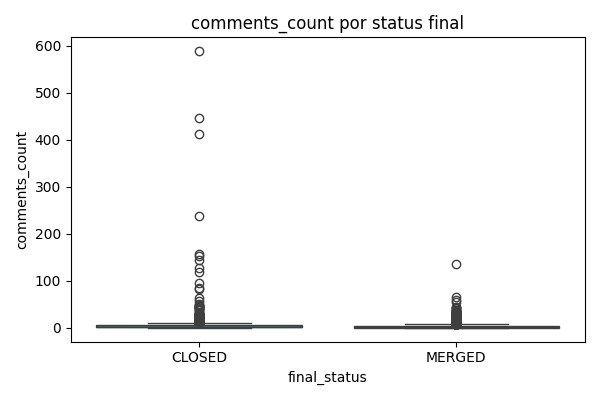
\includegraphics[width=\textwidth]{figs/box_comments_count.png}
    \caption{Comentários (***; MERGED $<$ CLOSED)}
  \end{subfigure}
  \caption{Distribuição por status (MERGED vs.\ CLOSED). Sig.: *** $p<0{,}001$. M\,=\,MERGED, C\,=\,CLOSED (cont.)}
  \label{fig:box4}
\end{figure}

\begin{itemize}
  \item \textbf{Arquivos alterados} --- diferença significativa (***): MERGED $>$ CLOSED.
  \item \textbf{Adições (linhas)} --- diferença significativa (***): MERGED $>$ CLOSED.
  \item \textbf{Deleções (linhas)} --- diferença significativa (***): MERGED $>$ CLOSED.
  \item \textbf{Tempo de revisão (h)} --- diferença significativa (***): MERGED $<$ CLOSED.
  \item \textbf{Tamanho da descrição} --- diferença significativa (***): MERGED $<$ CLOSED.
  \item \textbf{Participantes} --- diferença significativa (***): MERGED $<$ CLOSED.
  \item \textbf{Comentários} --- diferença significativa (***): MERGED $<$ CLOSED.
\end{itemize}

% ─────────────────────────────────────────────────────────────────────────────
\subsection{RQ$_B$ -- Relação entre características e número de revisões}
% ─────────────────────────────────────────────────────────────────────────────

A Tabela~\ref{tab:rqb} apresenta as correlações de Spearman com o número
de revisões. Todas as correlações são positivas e estatisticamente
significativas.

\begin{table}[H]
  \centering
  \caption{Correlações de Spearman com o número de revisões (todas positivas).}
  \label{tab:rqb}
  \small
  \begin{tabular}{lrl}
    \toprule
    \textbf{Métrica} & $\boldsymbol{\rho}$ & \textbf{Sig.} \\
    \midrule
    Arquivos alterados & 0,192 & *** \\
    Adições (linhas) & 0,210 & *** \\
    Deleções (linhas) & 0,106 & *** \\
    Tempo de revisão (h) & 0,118 & *** \\
    Tamanho da descrição & 0,199 & *** \\
    Participantes & 0,334 & *** \\
    Comentários & 0,305 & *** \\
    \bottomrule
  \end{tabular}
\end{table}

Os gráficos de dispersão abaixo mostram a relação de cada métrica com o
número de revisões. O valor de $\rho$ de Spearman e a significância
estão indicados em cada legenda:

\begin{figure}[H]
  \centering
  \begin{subfigure}[b]{0.48\columnwidth}
    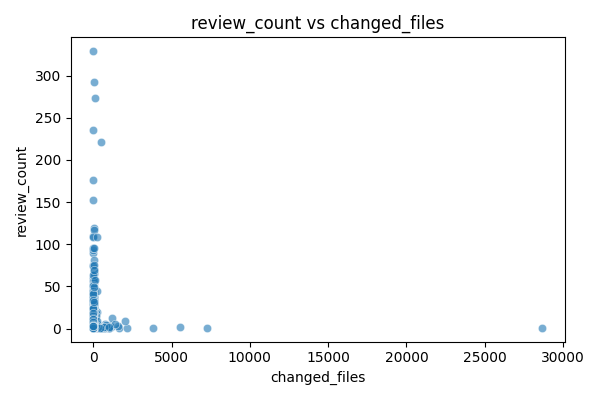
\includegraphics[width=\textwidth]{figs/scatter_reviews_changed_files.png}
    \caption{Arquivos alterados ($\rho=0,192$, ***)}
  \end{subfigure}
  \hfill
  \begin{subfigure}[b]{0.48\columnwidth}
    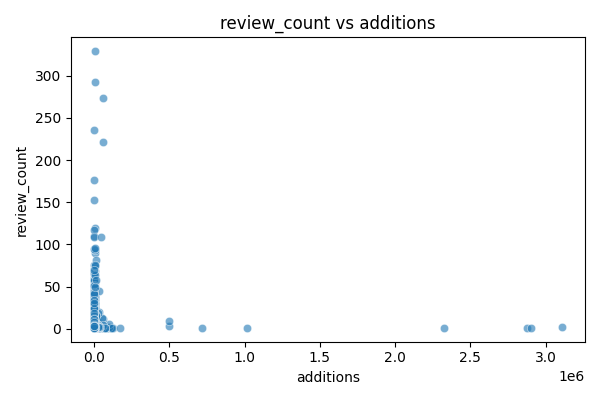
\includegraphics[width=\textwidth]{figs/scatter_reviews_additions.png}
    \caption{Adições (linhas) ($\rho=0,210$, ***)}
  \end{subfigure}
  \caption{Dispersão entre cada métrica e o número de revisões formais. Sig.: *** $p<0{,}001$}
  \label{fig:scat1}
\end{figure}

\begin{figure}[H]
  \centering
  \begin{subfigure}[b]{0.48\columnwidth}
    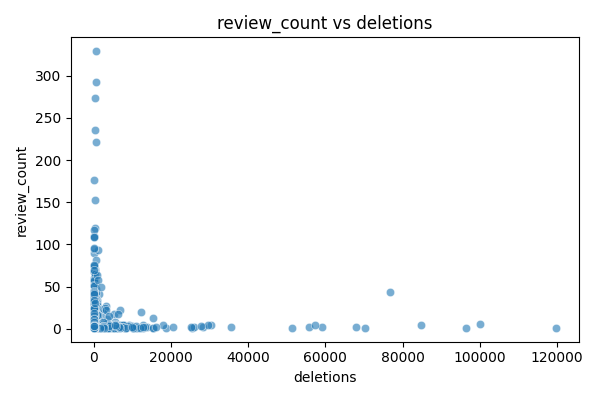
\includegraphics[width=\textwidth]{figs/scatter_reviews_deletions.png}
    \caption{Deleções (linhas) ($\rho=0,106$, ***)}
  \end{subfigure}
  \hfill
  \begin{subfigure}[b]{0.48\columnwidth}
    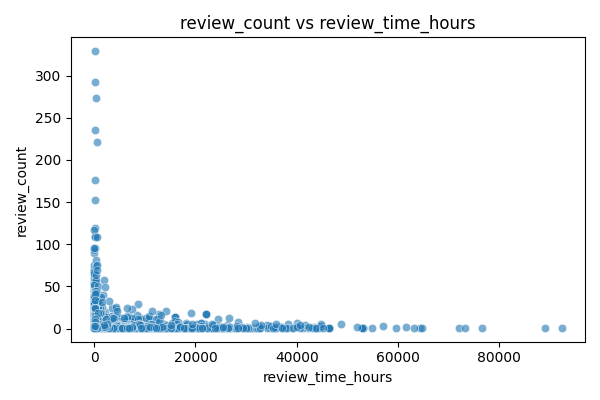
\includegraphics[width=\textwidth]{figs/scatter_reviews_review_time_hours.png}
    \caption{Tempo de revisão (h) ($\rho=0,118$, ***)}
  \end{subfigure}
  \caption{Dispersão entre cada métrica e o número de revisões formais. Sig.: *** $p<0{,}001$ (cont.)}
  \label{fig:scat2}
\end{figure}

\begin{figure}[H]
  \centering
  \begin{subfigure}[b]{0.48\columnwidth}
    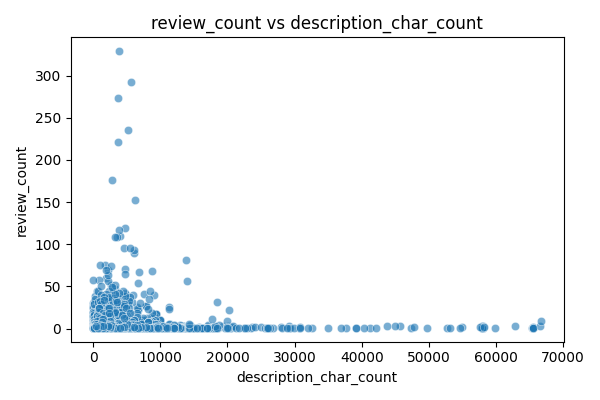
\includegraphics[width=\textwidth]{figs/scatter_reviews_description_char_count.png}
    \caption{Tamanho da descrição ($\rho=0,199$, ***)}
  \end{subfigure}
  \hfill
  \begin{subfigure}[b]{0.48\columnwidth}
    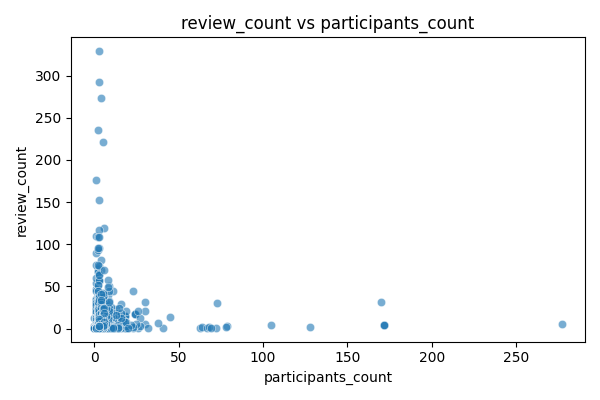
\includegraphics[width=\textwidth]{figs/scatter_reviews_participants_count.png}
    \caption{Participantes ($\rho=0,334$, ***)}
  \end{subfigure}
  \caption{Dispersão entre cada métrica e o número de revisões formais. Sig.: *** $p<0{,}001$ (cont.)}
  \label{fig:scat3}
\end{figure}

\begin{figure}[H]
  \centering
  \begin{subfigure}[b]{0.48\columnwidth}
    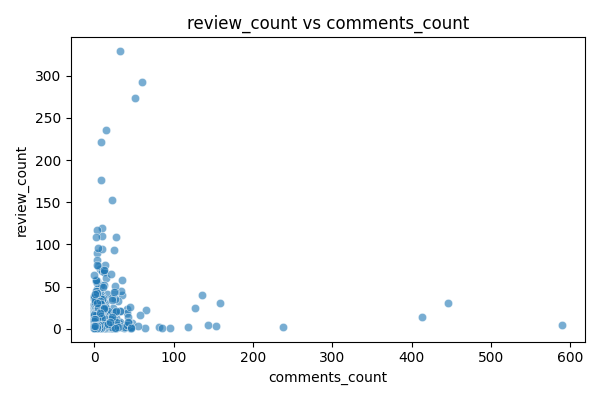
\includegraphics[width=\textwidth]{figs/scatter_reviews_comments_count.png}
    \caption{Comentários ($\rho=0,305$, ***)}
  \end{subfigure}
  \caption{Dispersão entre cada métrica e o número de revisões formais. Sig.: *** $p<0{,}001$ (cont.)}
  \label{fig:scat4}
\end{figure}

\begin{itemize}
  \item \textbf{Arquivos alterados} --- correlação fraca e positiva ($\rho = 0,192$, ***).
  \item \textbf{Adições (linhas)} --- correlação moderada e positiva ($\rho = 0,210$, ***).
  \item \textbf{Deleções (linhas)} --- correlação fraca e positiva ($\rho = 0,106$, ***).
  \item \textbf{Tempo de revisão (h)} --- correlação fraca e positiva ($\rho = 0,118$, ***).
  \item \textbf{Tamanho da descrição} --- correlação fraca e positiva ($\rho = 0,199$, ***).
  \item \textbf{Participantes} --- correlação moderada e positiva ($\rho = 0,334$, ***).
  \item \textbf{Comentários} --- correlação moderada e positiva ($\rho = 0,305$, ***).
\end{itemize}

% ─────────────────────────────────────────────────────────────────────────────
\section{Discussão dos Resultados}
% ─────────────────────────────────────────────────────────────────────────────

\subsection{Insights Principais}

\begin{itemize}
  \item \textbf{Diff menor favorece aprovação:} PRs MERGED apresentam, em
    mediana, menos arquivos alterados, adições e deleções. Mudanças de
    escopo reduzido são mais fáceis de revisar e têm maior taxa de
    aceitação.

  \item \textbf{PRs rejeitados ficam abertos por mais tempo:} o tempo de
    revisão é significativamente maior em PRs CLOSED, sugerindo que PRs
    problemáticos ficam estagnados ou que a demora desencoraja o autor.

  \item \textbf{Descrição importa:} PRs MERGED possuem descrições mais
    extensas, indicando que documentar adequadamente a mudança facilita
    a aprovação.

  \item \textbf{Engajamento impulsiona revisões:} participantes e
    comentários têm as maiores correlações com o número de revisões
    ($\rho \approx 0{,}33$ e $0{,}31$). Discussões mais ativas geram mais
    ciclos formais de revisão.

  \item \textbf{Tamanho do diff tem efeito moderado:} adições e tamanho
    da descrição correlacionam moderadamente ($\rho \approx 0{,}21$ e
    $0{,}20$); deleções e tempo de revisão têm efeito menor
    ($\rho \approx 0{,}11$).
\end{itemize}

\subsection{Implicações para Equipes de Desenvolvimento}

Os resultados sugerem práticas concretas: (i)~manter PRs pequenos e
focados aumenta a chance de aprovação; (ii)~descrições detalhadas
facilitam o processo de revisão; (iii)~engajar colaboradores nos
comentários aprofunda o ciclo formal de revisão.

% ─────────────────────────────────────────────────────────────────────────────
% Conclusão — mantida em duas colunas para fluxo contínuo com o restante.
% ─────────────────────────────────────────────────────────────────────────────
\section{Conclusão e Resposta às Hipóteses}
% ─────────────────────────────────────────────────────────────────────────────

A análise de 17.543 PRs dos repositórios mais populares do GitHub revelou que:

\begin{itemize}
  \item \textbf{Status final (RQ$_A$):} todas as métricas avaliadas
    apresentaram diferença estatisticamente significativa entre PRs MERGED
    e CLOSED. PRs aprovados tendem a ter diffs menores, descrições mais
    completas e menor tempo até o encerramento.
    A hipótese H$_A$ é \textbf{confirmada}.

  \item \textbf{Número de revisões (RQ$_B$):} as correlações mais fortes
    com o número de revisões são participantes e comentários, seguidos pelo
    tamanho do diff e da descrição. A hipótese H$_B$ é
    \textbf{confirmada}, especialmente quanto ao papel do engajamento.
\end{itemize}

\subsection{Tomadas de Decisão}

Com base nas evidências, recomendamos: (i)~limitar o escopo dos PRs para
facilitar revisão e aprovação; (ii)~investir em descrições que
contextualizem a mudança; (iii)~encorajar a participação de múltiplos
revisores desde o início; e (iv)~monitorar PRs com tempo de revisão
elevado como indicador de problemas de processo.

\subsection{Respondendo às Hipóteses}

A Tabela~\ref{tab:hipoteses} sintetiza o resultado de cada hipótese.

\begin{table}[H]
  \centering
  \caption{Síntese de confirmação das hipóteses.}
  \label{tab:hipoteses}
  \small
  \begin{tabularx}{\columnwidth}{lXl}
    \toprule
    Hip. & Descrição resumida & Status \\
    \midrule
    H$_A$ & PRs MERGED têm diffs menores e descrições mais completas. & Confirmada \\
    H$_B$ & Mais participantes e comentários $\Rightarrow$ mais revisões. & Confirmada \\
    \bottomrule
  \end{tabularx}
\end{table}

\end{document}
